%% Slides for ".NET Programming" by Chunyu Wang <chunyu@hit.edu.cn> %% -*- coding: utf-8 -*-

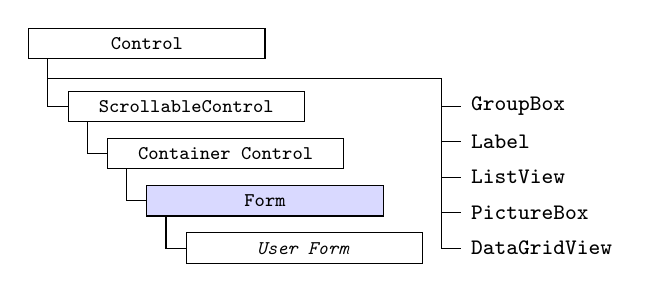
\begin{tikzpicture}
\tikzstyle{every node}=[anchor=west,font=\ttfamily\footnotesize]
\node at (5.5,4.4) (c1) {GroupBox};
\node at (5.5,3.95) (c2) {Label};
\node at (5.5,3.5) (c3) {ListView};
\node at (5.5,3.05) (c4) {PictureBox};
\node at (5.5,2.6) (c5) {DataGridView};

\tikzstyle{every node}=[anchor=west,draw,minimum width=3cm,fill=white,font=\ttfamily\scriptsize]
\node at (0,5.2) (a) {\textbf{Control}};
\node at (.5,4.4) (b) {ScrollableControl};
\node at (1,3.8) (b1) {Container Control};
\node[fill=blue!15] at (1.5,3.2) (b2) {Form};
\node at (2,2.6) (b3) {\textit{User Form}};

\draw (a.south west) +(right:.25cm) |- (b);
\draw (b.south west) +(right:.25cm) |- (b1);
\draw (b1.south west) +(right:.25cm) |- (b2);
\draw (b2.south west) +(right:.25cm) |- (b3);

\draw (.25,4.75) -- (5.25,4.75);

\foreach \a in {c1,c2,c3,c4,c5}
\draw (5.25,4.75) |- (\a);
\end{tikzpicture}
